\chapter{Understanding and Extending GrGen.NET}\indexmain{internals}\indexmain{Developing GrGen.NET} \label{cha:developing}

This chapter describes the inner workings of \GrG~to allow external developers
\begin{itemize}
\item to understand how \GrG~works, just out of curiosity or in order to optimize their code
\item extend \GrG~with new features, maybe being of general interest, maybe being only special extensions not of interest to other users
\end{itemize}

%%%%%%%%%%%%%%%%%%%%%%%%%%%%%%%%%%%%%%%%%%%%%%%%%%%%%%%%%%%%%%%%%%%%%%%%%%%%%%%%%%%%%%%%%%%%%%%%
\section{How to build}\label{sub:building}\indexmain{building GrGen}

In case you want to build \GrG~on your own you should recall the system layout \ref{figsys}. 
The graph rewrite generator consists of a frontend written in Java and a backend written in C\#.
The frontend was extended and changed since its first version, but not replaced.
In contrast to the backend, which has seen multiple engines and versions: a MySQL database based version, a PSQL database based version, 
a C version executing a search plan with a virtual machine, a C\# engine executing code generated from a search plan and finally the current C\# engine version 2 capable of matching nested and subpatterns.
The frontend is available in the \texttt{frontend} subdirectory of the public mercurial repository at \texttt{https://bitbucket.org/eja/grgen}.
It can be built with the included \texttt{Makefile} on Linux or the \texttt{Makefile\_Cygwin} on Windows with the cygwin environment yielding a \texttt{grgen.jar}. 
Alternatively you may add the \texttt{de} subfolder and the jars in the \texttt{jars} subfolder to your favourite IDE, but then you must take care of the ANTLR parser generation pre-build-step on your own. 
The backend is available in the \texttt{engine-net-2} subdirectory. 
It contains a VisualStudio 2008 solution file containing projects for the \texttt{libGr}, the \texttt{lgspBackend} (libGr-Search-Plan-Backend) and the \texttt{GrShell}.
Before you can build the solution you must execute \texttt{./src/libGr/genparser.bat}, \texttt{./src/libGr/GRSImporter/genparser.bat} and \texttt{./src/Gr\-Shell/genparser.bat}
to get the CSharpCC parsers for the rewrite sequences, the GRS importer and the shell generated.
Under LINUX you may use \texttt{make\_linux.sh} to get a complete build.
To get the API examples generated you must execute \texttt{./genlibs.bat}.
The \texttt{doc} subdirectory contains the sources of the user manual, for building say \texttt{./build\_cygwin.sh grgen} on Windows in \texttt{cygwin-bash} or \texttt{./build grgen} on Linux in \texttt{bash}.
The \texttt{syntaxhighlighting} subdirectory contains syntax highlighting specifications for the GrGen-files for \texttt{Notepad++} and \texttt{vim}.

You can check the result of your build with the test suite we use to check against regressions.
It is split into syntactic tests in \texttt{frontend/test} checking that example model and rule files can get compiled by \texttt{grgen} (or not compiled, or only compiled emitting warnings) and the resulting code can get compiled by \texttt{csc}.
The tests get executed by calling \texttt{./test.sh} or \texttt{./testpar.sh} from \texttt{bash} or \texttt{cygwin-bash} (\texttt{testpar.sh} executes them in parallel speeding up execution on multi core systems considerably at the price of potential false positive reports); deviations from a gold standard are reported.
And semantic tests in \texttt{engine-net-2/tests} checking that executing example shell scripts on example models and rules yields the expected results. 
They get executed by calling \texttt{./test.sh}.


%%%%%%%%%%%%%%%%%%%%%%%%%%%%%%%%%%%%%%%%%%%%%%%%%%%%%%%%%%%%%%%%%%%%%%%%%%%%%%%%%%%%%%%%%%%%%%%%
\section{The concepts behind the code generation and the generated code}
todo: Merge with tour of the code, explain code together with generated code?
Or better: split into explaining concepts of what is generated of general interest to users
and explaining code generation, how it work, only of interest for people which want to extend grgen?

Model:
The graph structure is maintained in the LGSPGraph built of LGSPNode and LGSPEdge objects without type and attribute information. The generated node and edge interfaces defining the user visible types and attributes are implemented by generated node and edge classes inheriting from and working like LGSPNodes and LGSPEdges in the LGSPGraph, additionally implementing the type and attribute bearing interfaces.

\begin{figure}[htbp]
  \centering
  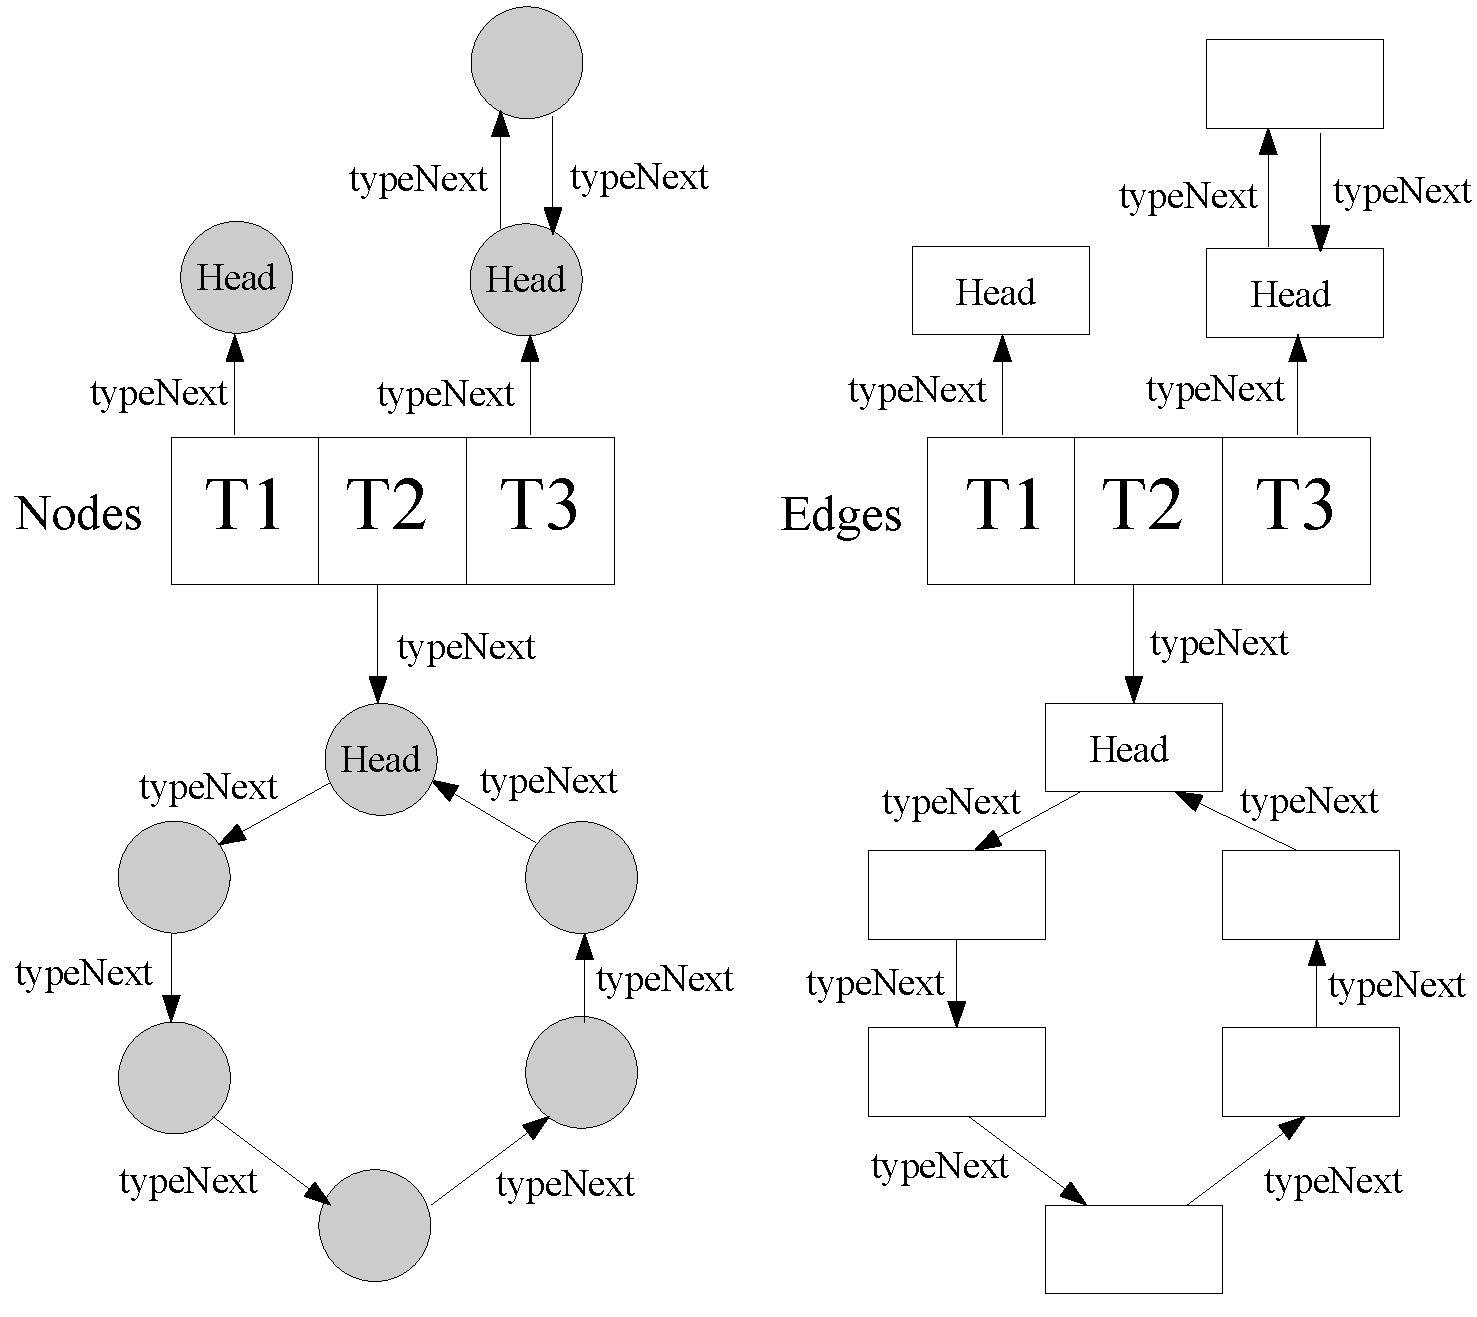
\includegraphics[width=0.7\textwidth]{fig/TypeRinglists}
  \caption{Example for type ringlists}
  \label{figtyperinglists}
\end{figure}

\begin{figure}[htbp]
  \centering
  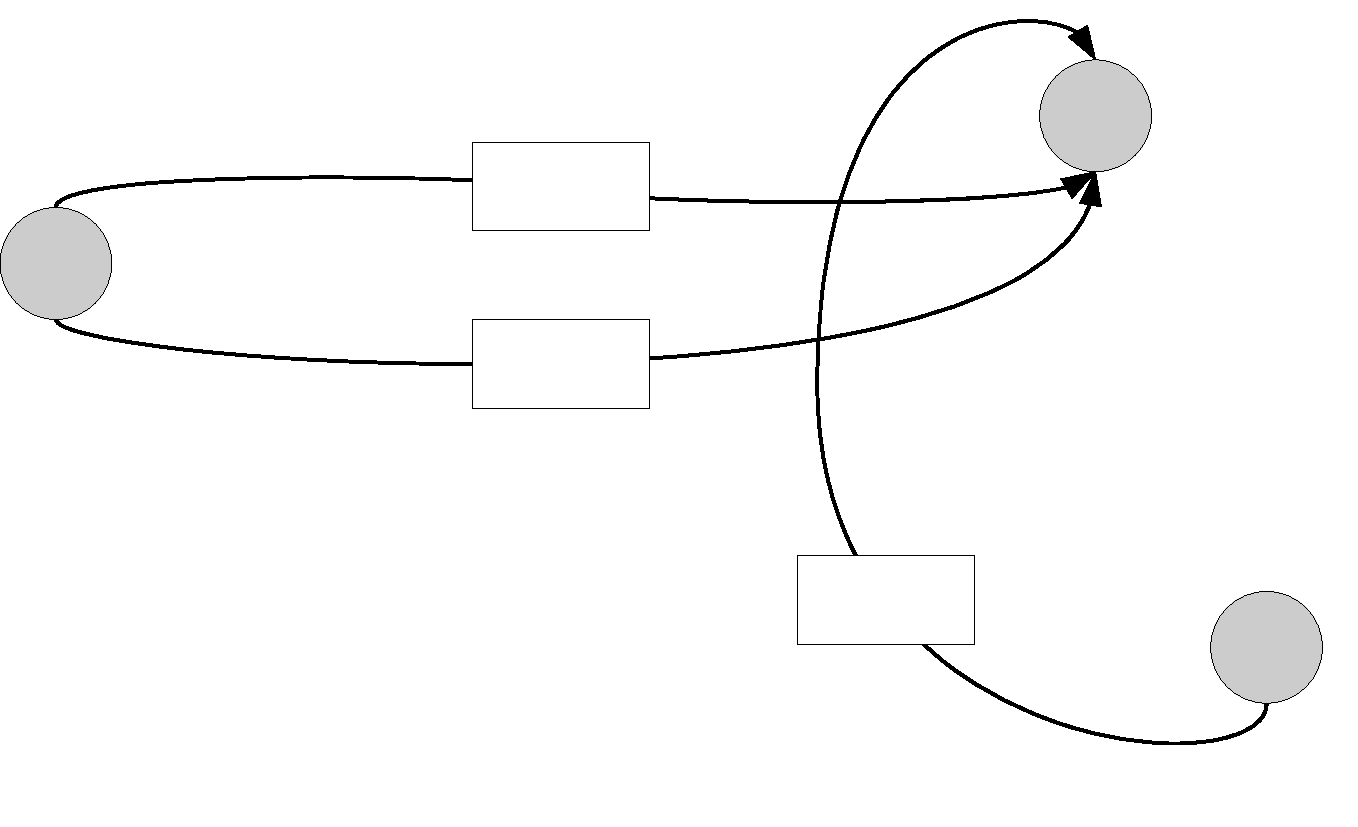
\includegraphics[width=\textwidth]{fig/IncidenceExample}
  \caption{Incidence example situation}
  \label{figincidenceexample}
\end{figure}

\begin{figure}[htbp]
  \centering
  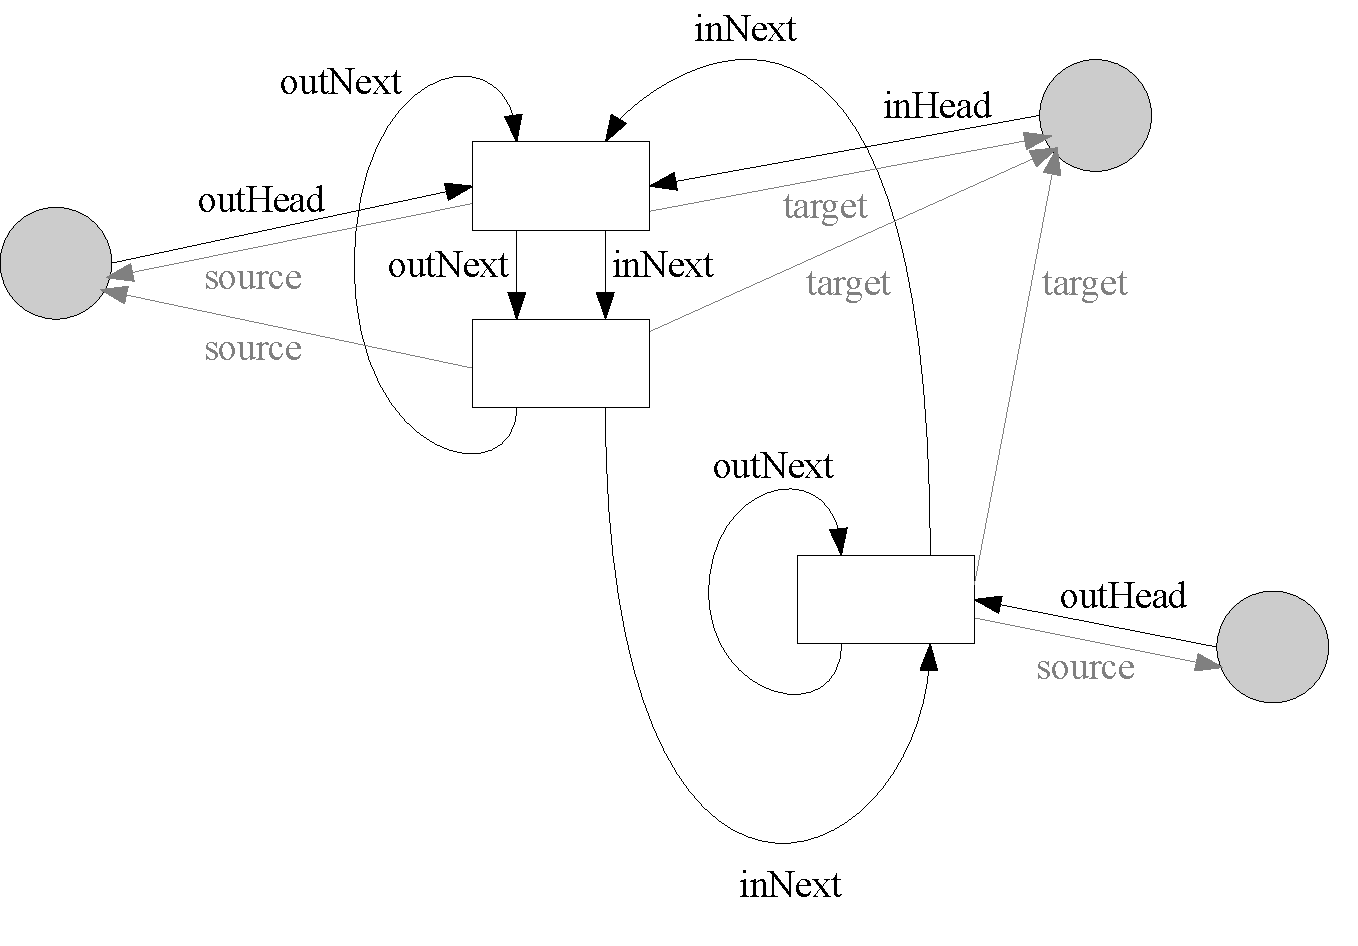
\includegraphics[width=\textwidth]{fig/IncidenceExampleRinglists}
  \caption{Ringlist implementation of incidence example}
  \label{figincidenceexampleringlists}
\end{figure}


Pattern Search planning: Search plan lowered into more detailed search program.
Why search planning? vstructures, splitting; example 1 bad, example 2 good

\begin{figure}[htbp]
  \centering
  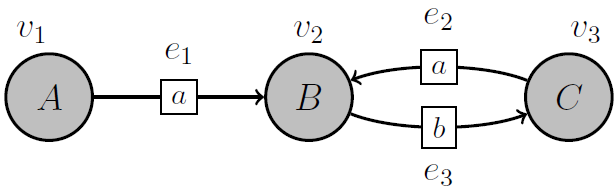
\includegraphics[width=\textwidth]{fig/Pattern}
  \caption{Pattern to search}
  \label{figpatterntosearch}
\end{figure}

\begin{figure}[htbp]
  \centering
  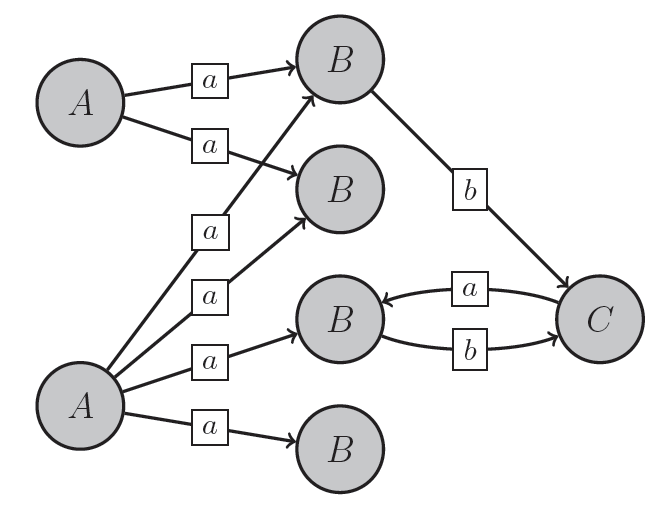
\includegraphics[width=\textwidth]{fig/Graph}
  \caption{Host graph to search in}
  \label{figgraphtosearchin}
\end{figure}

\begin{figure}[htbp]
  \centering
  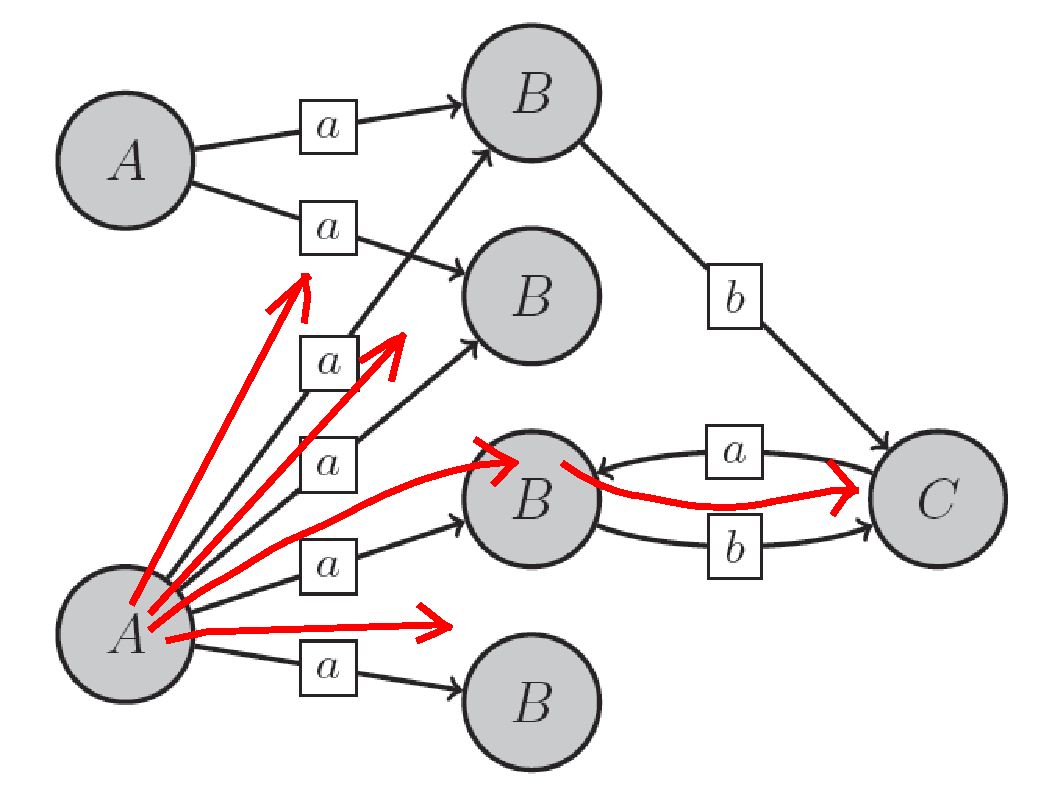
\includegraphics[width=\textwidth]{fig/GraphBad}
  \caption{Bad search order}
  \label{figbadsearch}
\end{figure}

\texttt{lkp(v1:A); out(v1,e1:a); tgt(e1,v2:B);}\\
\texttt{out(v2,e3:b); tgt(e3,v3:C); out(v3,e2:a); tgt(e2,v2:B)}

\begin{csharp}
foreach(v1:A in graph) {
	foreach(e1 in outgoing(v1)) {
		if(type(e1)!=a) continue;
		v2 = e1.tgt;
		if(type(v2)!=B) continue;
		foreach(e3 in outgoing(v2)) {
			if(type(e3)!=b) continue;
			v3 = e3.tgt;
			if(type(v3)!=C) continue;
			foreach(e2 in outgoing(v3)) {
				if(type(e2)!=a) continue;
				if(e2.tgt!=v2) continue;
				// v1,e1,v2,e3,v3,v2 constitute a match
			} 
		}
	}
}
\end{csharp}

\begin{figure}[htbp]
  \centering
  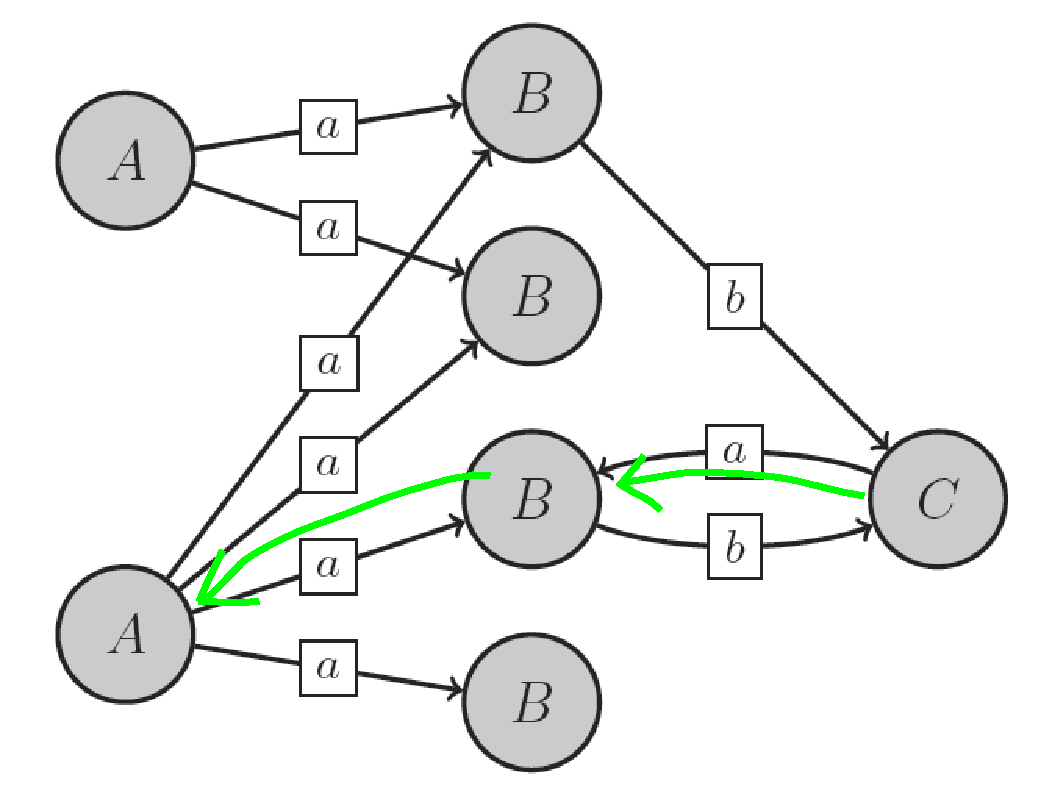
\includegraphics[width=\textwidth]{fig/GraphGood}
  \caption{Good search order}
  \label{figgoodsearch}
\end{figure}

\texttt{lkp(v3:C); out(v3,e2:a); tgt(e2,v2:B);}\\
\texttt{out(v2,e3:b); tgt(e3,v3:C); in(v2,e1:a); src(e1,v1:A)}

\begin{csharp}
foreach(v3:C in graph) {
	foreach(e2 in outgoing(v3)) {
		if(type(e2)!=a) continue;
		v2 = e2.tgt;
		if(type(v2)!=B) continue;
		foreach(e3 in outgoing(v2)) {
			if(type(e3)!=b) continue;
			if(e3.tgt!=v3) continue;
				foreach(e1 in incoming(v2)) {
				if(type(e1)!=a) continue;
				v1 = e1.src;
				if(type(v1)!=A) continue;
				// v3,e2,v2,e3,e1,v1 constitute a match
			} 
		}
	}
}
\end{csharp}

\begin{note}
Corollary from what you've seen: Use types!

less to search on lookup
faster leaving (continue)
better statistics

search plans:
use runtime statistics
can give static priorities
\end{note}

Search program:
connectedness, isomorphy checks
Patterns built from pieces:

\pagebreak

\begin{figure}[htbp]
  \centering
  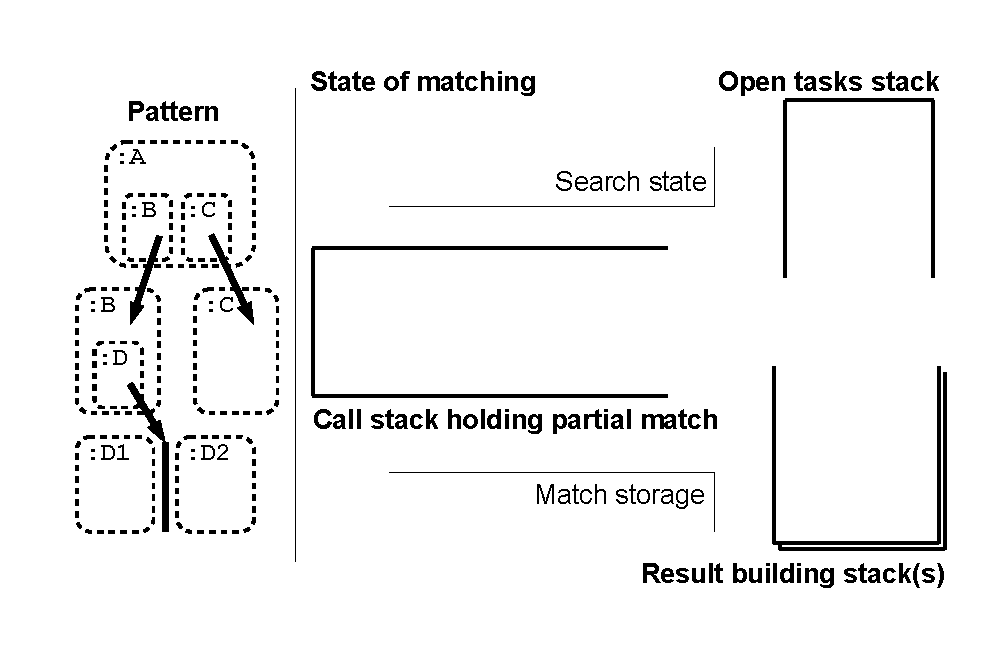
\includegraphics[width=\textwidth]{fig/Passungszustand1}
  \caption{todo}
  \label{figmatchingstate1}
\end{figure}

\begin{figure}[htbp]
  \centering
  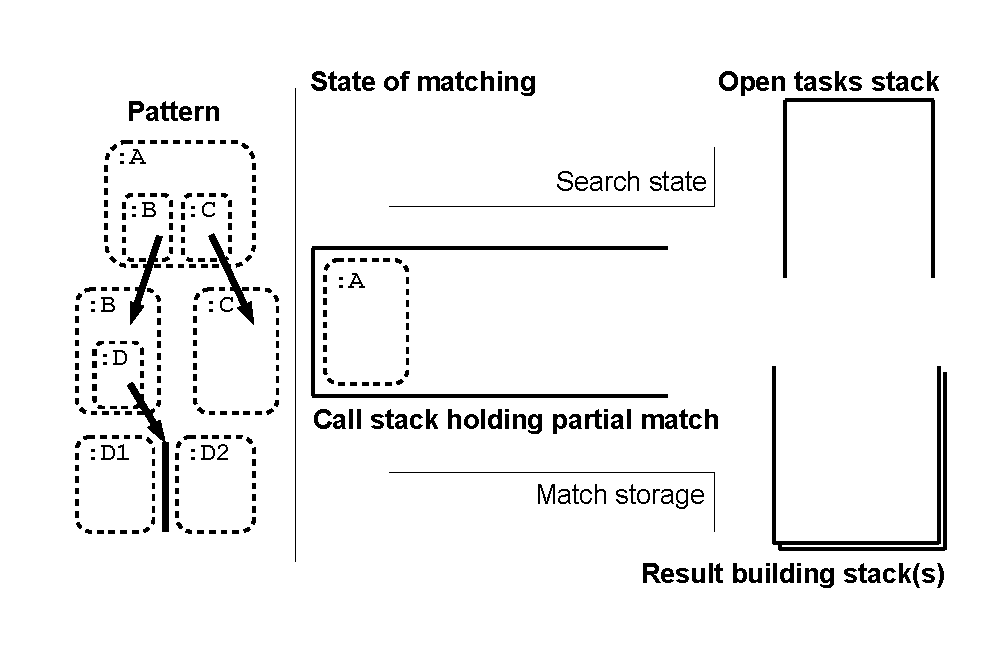
\includegraphics[width=\textwidth]{fig/Passungszustand2}
  \caption{todo}
  \label{figmatchingstate2}
\end{figure}

\begin{figure}[htbp]
  \centering
  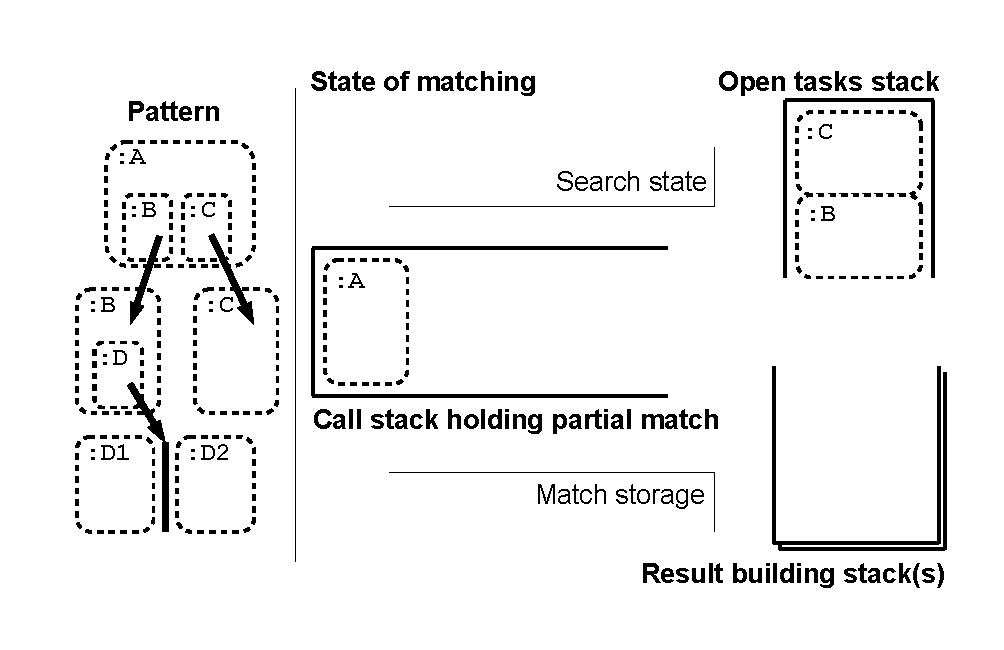
\includegraphics[width=\textwidth]{fig/Passungszustand3}
  \caption{todo}
  \label{figmatchingstate3}
\end{figure}

\begin{figure}[htbp]
  \centering
  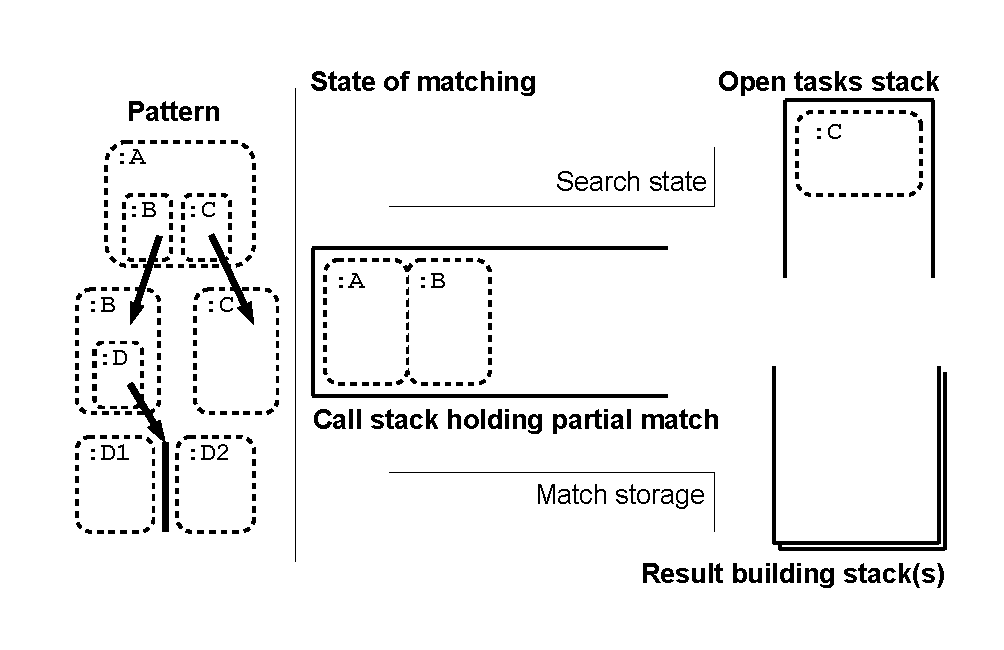
\includegraphics[width=\textwidth]{fig/Passungszustand4}
  \caption{todo}
  \label{figmatchingstate4}
\end{figure}

\begin{figure}[htbp]
  \centering
  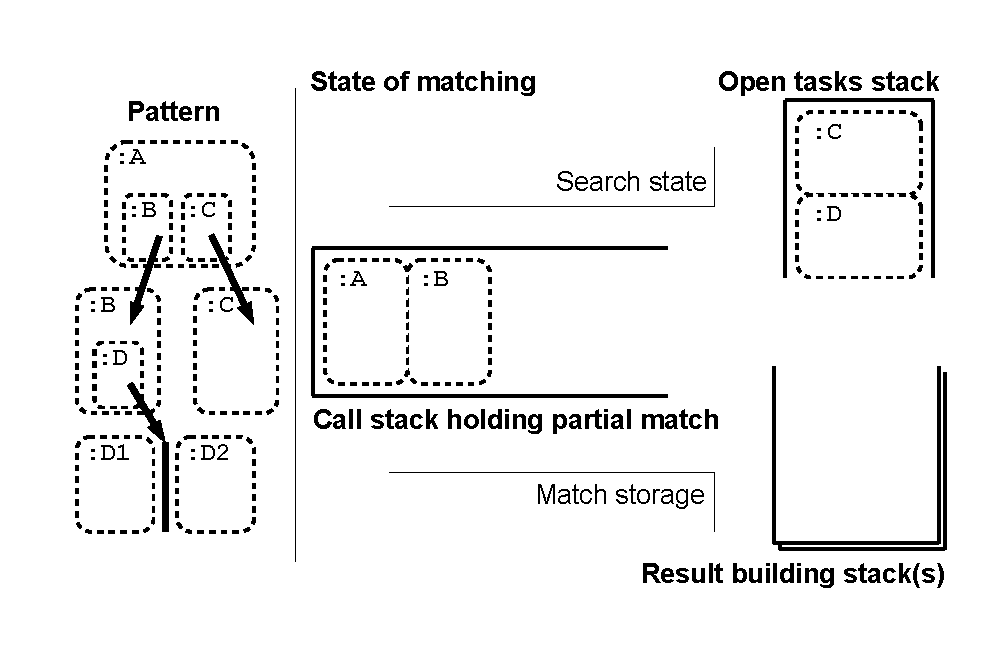
\includegraphics[width=\textwidth]{fig/Passungszustand5}
  \caption{todo}
  \label{figmatchingstate5}
\end{figure}

\begin{figure}[htbp]
  \centering
  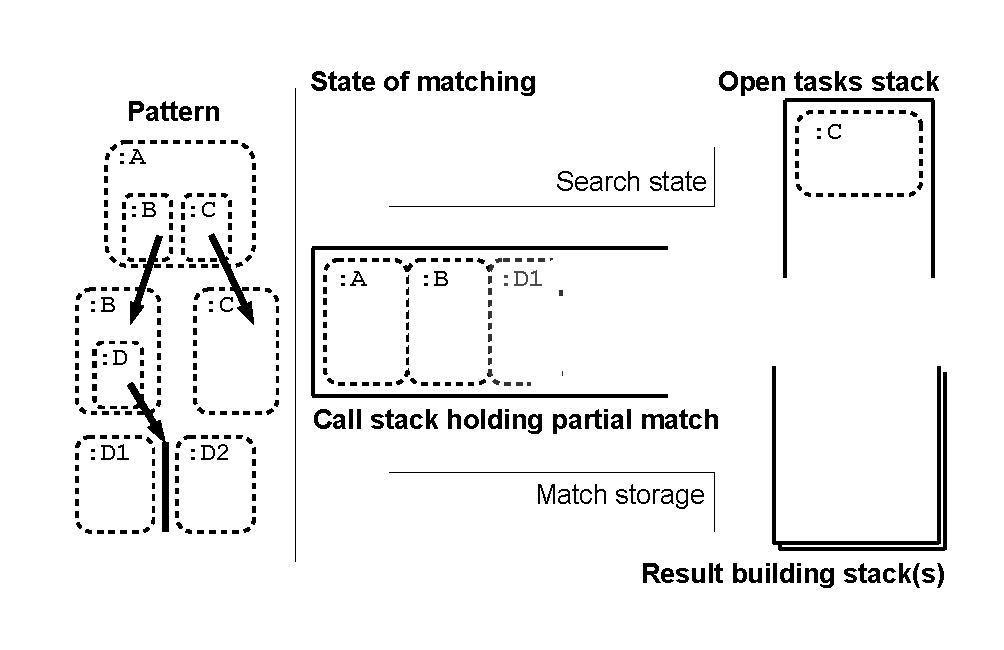
\includegraphics[width=\textwidth]{fig/Passungszustand6}
  \caption{todo}
  \label{figmatchingstate6}
\end{figure}

\begin{figure}[htbp]
  \centering
  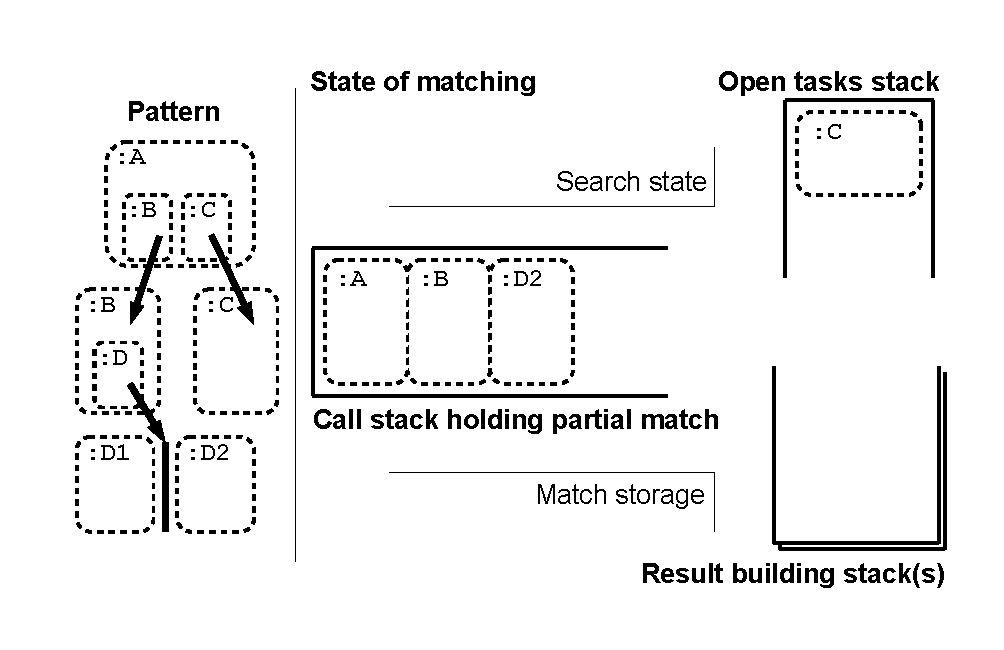
\includegraphics[width=\textwidth]{fig/Passungszustand7}
  \caption{todo}
  \label{figmatchingstate7}
\end{figure}

\begin{figure}[htbp]
  \centering
  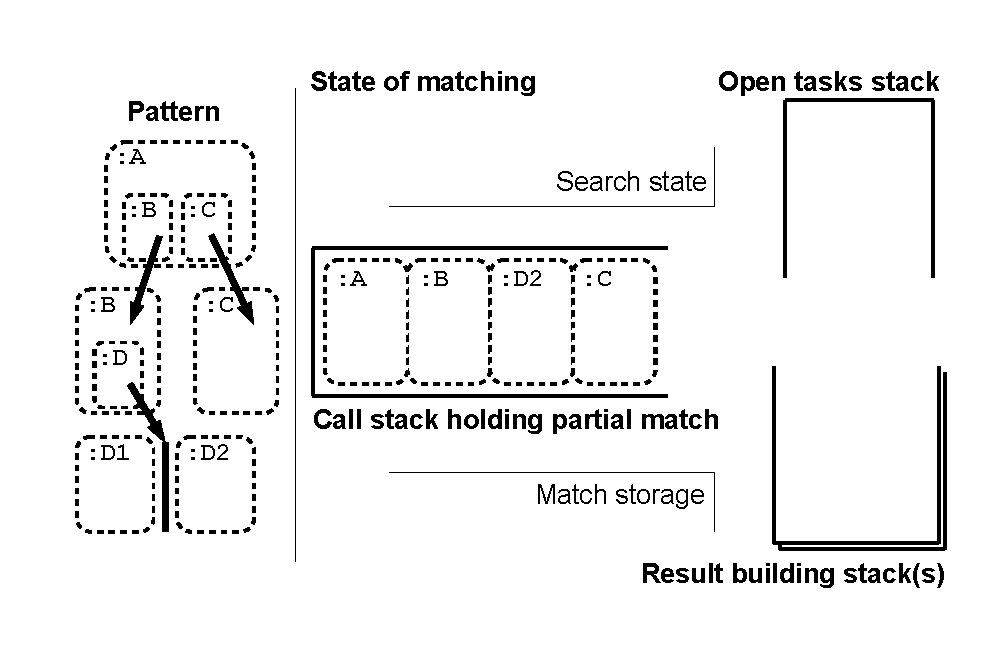
\includegraphics[width=\textwidth]{fig/Passungszustand8}
  \caption{todo}
  \label{figmatchingstate8}
\end{figure}

\begin{figure}[htbp]
  \centering
  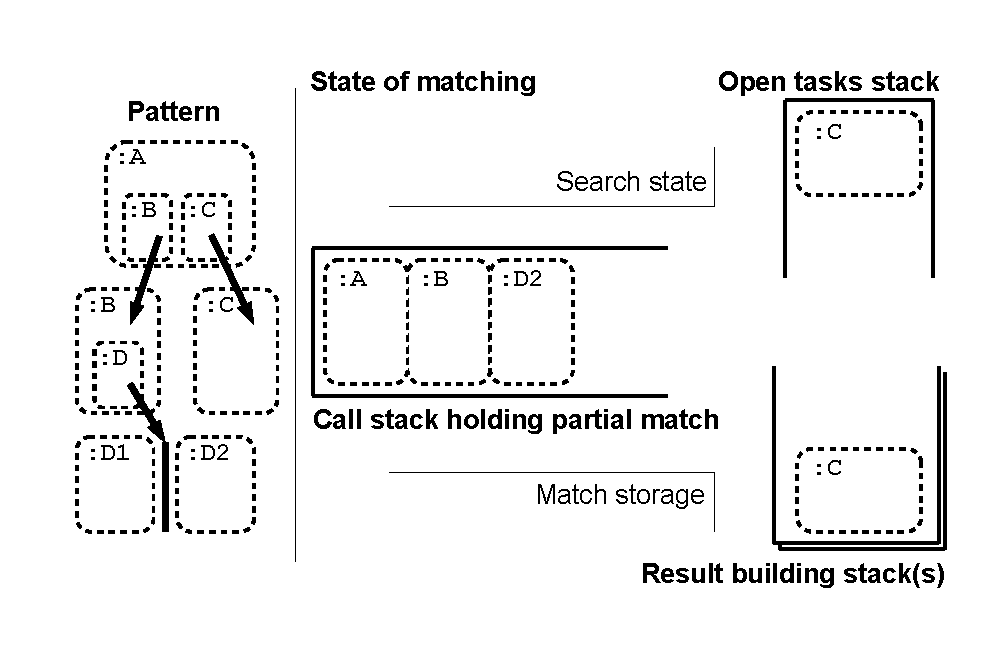
\includegraphics[width=\textwidth]{fig/Passungszustand9}
  \caption{todo}
  \label{figmatchingstate9}
\end{figure}

\begin{figure}[htbp]
  \centering
  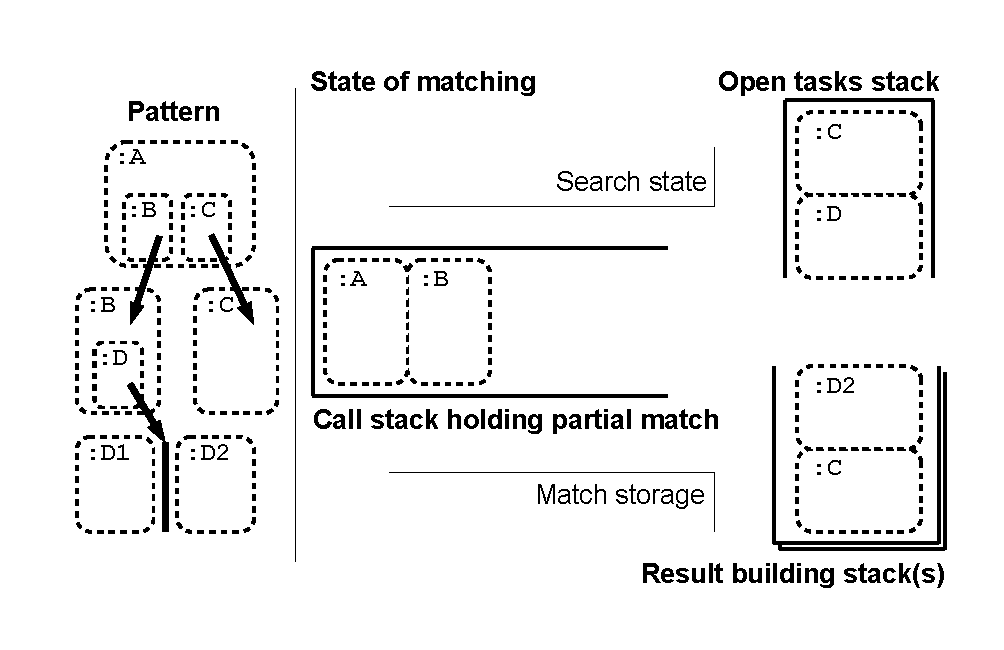
\includegraphics[width=\textwidth]{fig/Passungszustand10}
  \caption{todo}
  \label{figmatchingstate10}
\end{figure}

\begin{figure}[htbp]
  \centering
  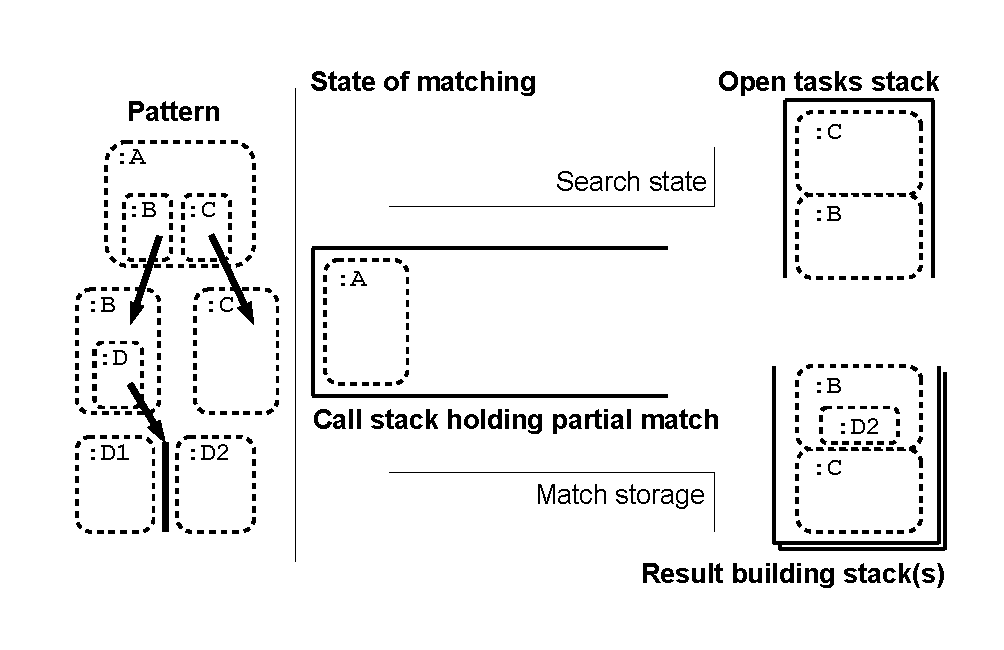
\includegraphics[width=\textwidth]{fig/Passungszustand11}
  \caption{todo}
  \label{figmatchingstate11}
\end{figure}

\begin{figure}[htbp]
  \centering
  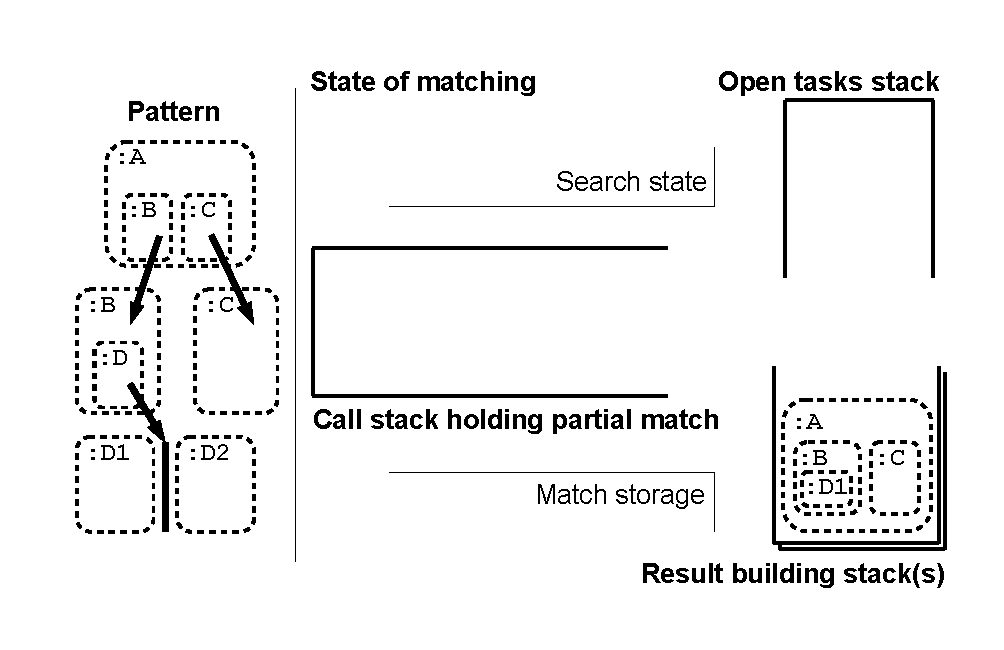
\includegraphics[width=\textwidth]{fig/Passungszustand12}
  \caption{todo}
  \label{figmatchingstate12}
\end{figure}


%%%%%%%%%%%%%%%%%%%%%%%%%%%%%%%%%%%%%%%%%%%%%%%%%%%%%%%%%%%%%%%%%%%%%%%%%%%%%%%%%%%%%%%%%%%%%%%%
\section{A short tour of the code}

\begin{figure}[htbp]
  \centering
  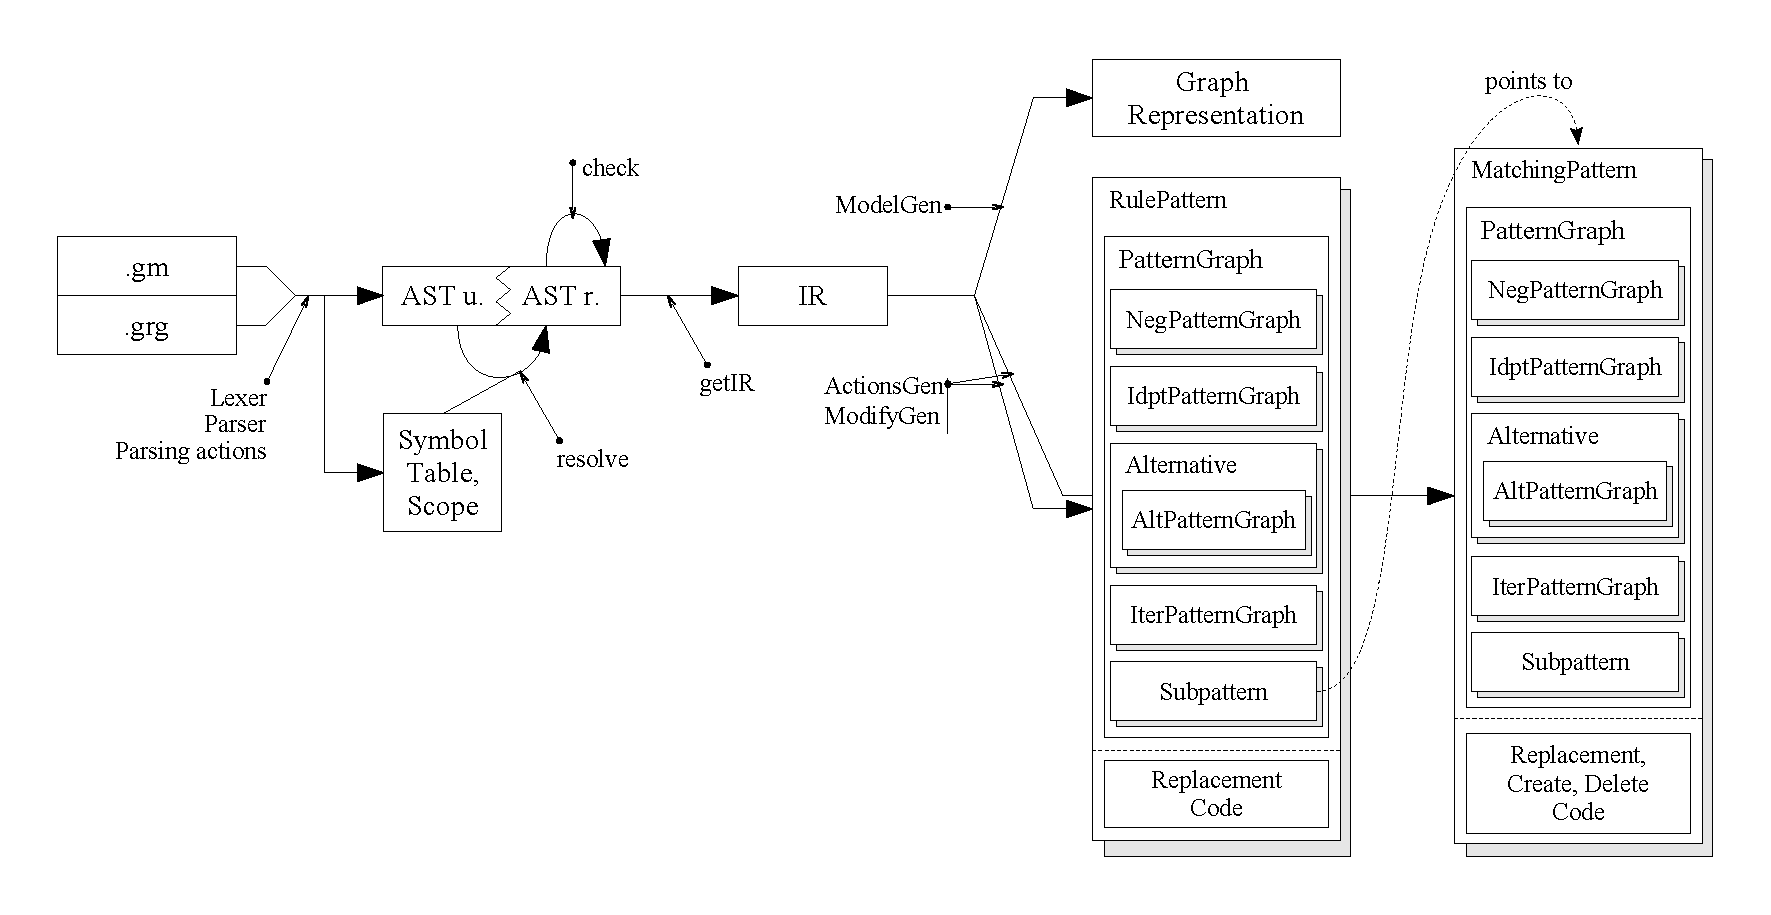
\includegraphics[width=\textwidth]{fig/AblaufCodeerzeugungFrontend}
  \caption{Frontend Code Generation}
  \label{figfrontendcodegen}
\end{figure}

The frontend is spread over the directories \texttt{parser}, \texttt{ast}, \texttt{ir}, \texttt{be} and \texttt{util}, with their code being used from \texttt{Main.java}.
The directory \texttt{parser} contains parser helpers like the symbol table and scopes and within the \texttt{antlr} subdirectory the ANTLR parser grammar of \GrG~in the file \texttt{Grgen.g}.
The semantic actions of the parser build an abstract syntax tree consisting of instances of a multiple classes as given in the directory \texttt{ast}, with the base class \texttt{BaseNode}.
The AST is operated upon in three passes, first resolving by \texttt{resolve} and \texttt{resolveLocal}, mainly replacing identifier nodes by their declaration nodes in an (largely) preorder walk.
Afterwards the AST is checked by \texttt{check} and \texttt{checkLocal} in an (largely) postorder walk for type and other semantic constraints.
Finally an intermediate representation is built from the abstract syntax tree by the \texttt{getIR} and \texttt{constructIR} methods.
The IR classes given in the \texttt{ir} folder can be seen as more lightweight AST classes; their name is often the same as for their corresponding AST classes, but without the \texttt{Node}-suffix which is appended to all AST classes.
The IR classes are the input to the two backends of the frontend, as given in the folders \texttt{be/C} and \texttt{be/Csharp}.
The directory \texttt{be/C} contains the code generator for the C based backend integrated into the IPD C compiler.
(The compiler transforms a C program into a graph and SSA based compiler intermediate representation named FIRM using libFirm (see \url{libfirm.org}, \cite{TBL:99}, \cite{Lin:02}) and further on to x86 machine code.)
The directory \texttt{be/Csharp} contains the code generator for the C\# based backend of \GrG. 
It generates the model source code \texttt{FooModel.cs} with the node and edge classes for a rule file named \texttt{Foo.grg}, 
and the intermediate rules source code \texttt{FooActions\_intermediate} with a description of the patterns to match, a description of the embedded graph rewrite sequences, and the rewriting code.
It does \emph{not} generate the complete rules source code with the matcher code or the code for the embedded rewrite sequences, this is done by \texttt{grgen.exe} which only calls the \texttt{grgen.jar} of the frontend.
You may call the Java archive on your own to get a visualization of the model and rewrite rules from a \texttt{.vcg}-dump of the IR, cf. Note\ref{note:modelruledump}.


\begin{figure}[htbp]
  \centering
  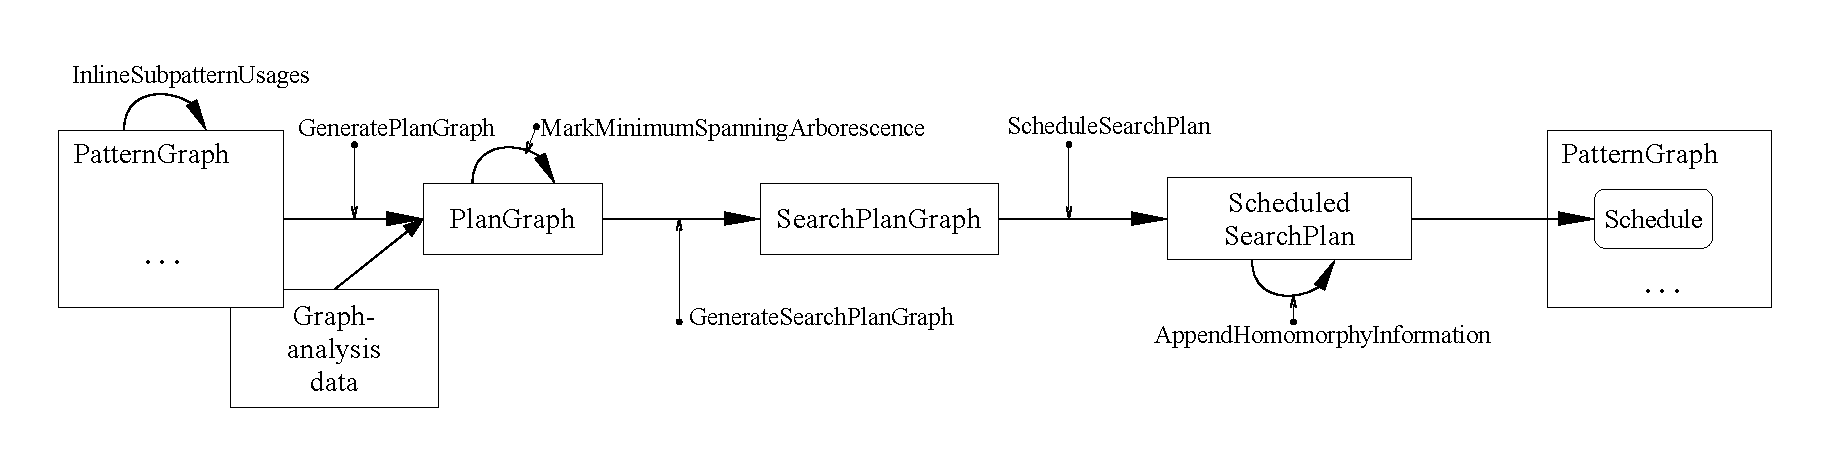
\includegraphics[width=\textwidth]{fig/AblaufCodeerzeugungBackend1}
  \caption{Backend Code Generation, step 1}
  \label{figbackendcodegen1}
\end{figure}

\begin{figure}[htbp]
  \centering
  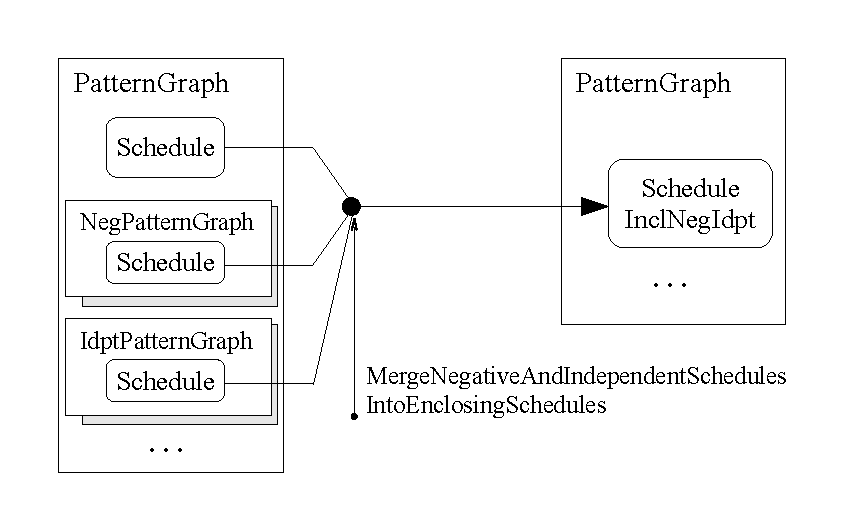
\includegraphics[width=\textwidth]{fig/AblaufCodeerzeugungBackend2}
  \caption{Backend Code Generation, step 2}
  \label{figbackendcodegen2}
\end{figure}

\begin{figure}[htbp]
  \centering
  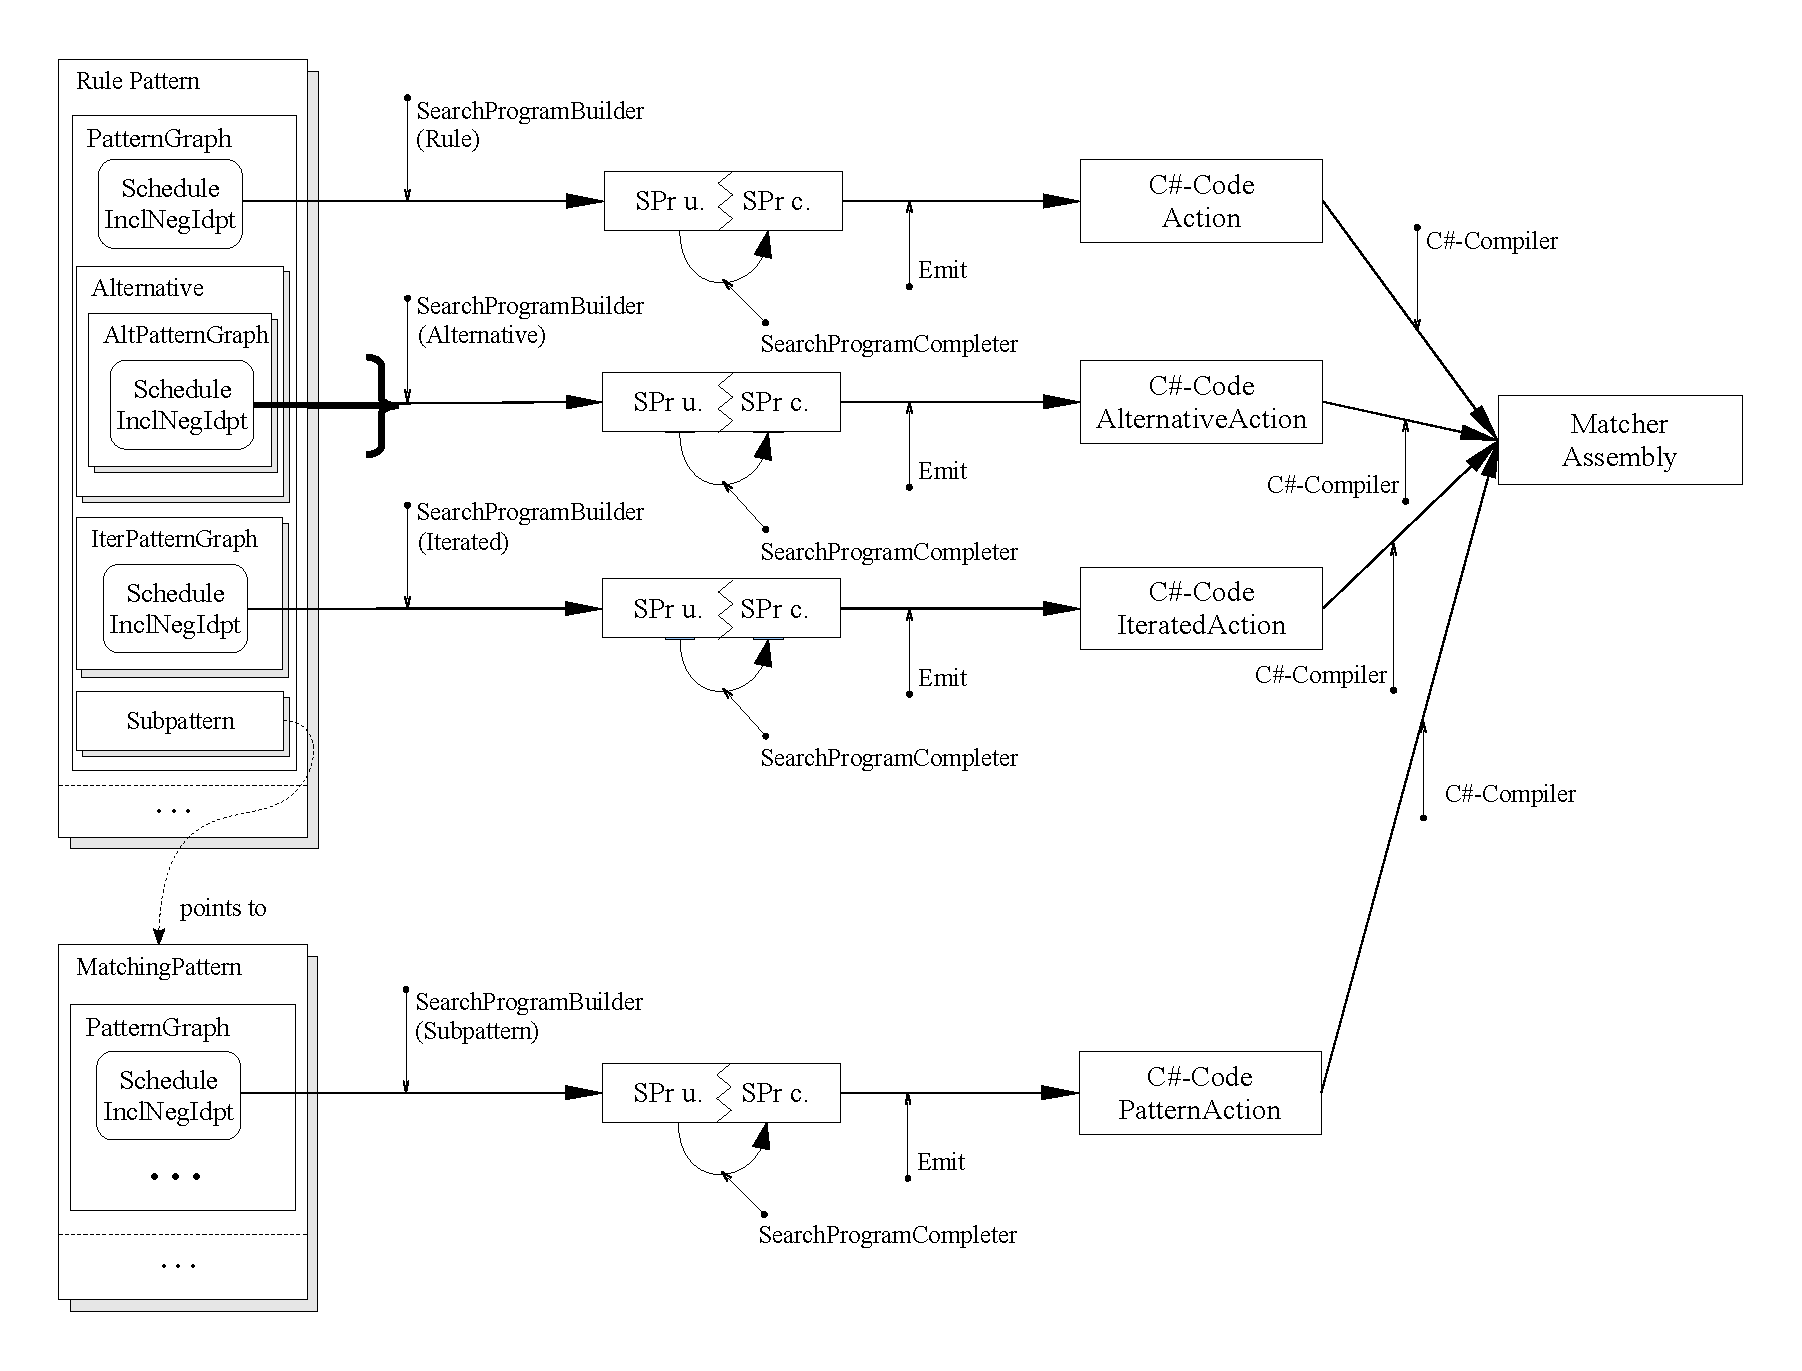
\includegraphics[width=\textwidth]{fig/AblaufCodeerzeugungBackend3}
  \caption{Backend Code Generation, step 3}
  \label{figbackendcodegen3}
\end{figure}

The real matcher code is generated by the backend given in \texttt{engine-net-2}, in the \texttt{src/lgspBackend} subdirectory.
The processing is done in several passes in \texttt{lgsp\-Matcher\-Generator.cs}; the base data structure is the \texttt{PatternGraph}, resp. the nesting of the \texttt{PatternGraph}-objects contained in the \texttt{RulePattern}-objects of the rules/tests or the \texttt{Matching\-Pattern}-objects of the subpatterns.
First a \texttt{PlanGraph} is created from the \texttt{PatternGraph} and data from analysing the host graph (for generating the initial matcher some default data given from the frontend is used).
A mimimum spanning arborescent is searched defining a hopefully optimal set of operations for matching the pattern (the hopes are founded, see \cite{BKG:07}).
A \texttt{SearchPlanGraph} is built from the arborescent marked in the \texttt{PlanGraph} and used thereafter for scheduling the operations into a \texttt{ScheduledSearchPlan}.
Out of the \texttt{ScheduledSearchPlan} a \texttt{SearchProgram} is built by the \texttt{SearchProgramBuilder};
in a further pass the \texttt{SearchProgram} is completed by the \texttt{SearchProgramCompleter},
before the C\# code gets finally generated by calling the \texttt{emit} methods of the \texttt{SearchProgram}.
The compiled graph rewrite sequences are handled by the \texttt{lgspSequenceChecker} and \texttt{lgspSequenceGenerator} (together with the sequence parser from the libGr).
The \texttt{src/GrGen} subdirectory contains the \texttt{grgen.exe} compiler driver procedure.
The \texttt{src/libGr} subdirectory contains the libGr, offering the base interfaces a user of \GrG~sees on the API level for the model, the actions, the pattern graphs and the host graph.
They get implemented in code from the lgsp backend and in the generated code.
The libGr further offers a generic, name string and object based interface to access the named entities of the generated code.
In addition it offers the rewrite sequence parser which gets generated out of \texttt{SequenceParser.csc},
building the rewrite sequence AST from the classes in \texttt{Sequence.cs} further utilizing \texttt{SymbolTable.cs}.
The rewrite sequence classes contain a method \texttt{ApplyImpl(IGraph graph)} which executes them.
Finally the libGr offers several importers and exporters in the \texttt{src/libGr/IO} and \texttt{src/libGr/GRSImporter} subfolders.
The \texttt{src/GrShell} subdirectory contains the GrShell application, which builds upon the generic interface (as it must be capable of coping with arbitrary used defined models and actions at runtime) and the sequence interpretation facilities offered by the libGr.
The command line parser of GrShell gets generated out of \texttt{GrShell.csc}, the shell implementation is given in \texttt{GrShellImpl.cs}.
Graphical debugging is offered by the \texttt{Debugger.cs} together with the \texttt{YCompClient.cs}.
The \texttt{examples} subdirectory of \texttt{engine-net-2} contains a bunch of examples for using \GrG~with GrShell.
The \texttt{examples-api} subdirectory contains several examples of how to use \GrG~from the API.
In case you want to contribute and got further questions don't hesitate to contact us 
(via email to \texttt{grgen} at the host given by \texttt{ipd.info.uni-karlsruhe.de}).


%\section{How the search plan backend works / How to optmize}
%host graph sensitive search plan driven graph pattern matching, 2+n pushdown machine, code generator
%graph data structure, type list, incidence list, pattern matcher loops iterating lists
%-> optimize: use types eagerly;  generate search plans at runtime

